\documentclass{standalone}
\usepackage{tikz}
\usetikzlibrary{patterns, positioning}


\begin{document}
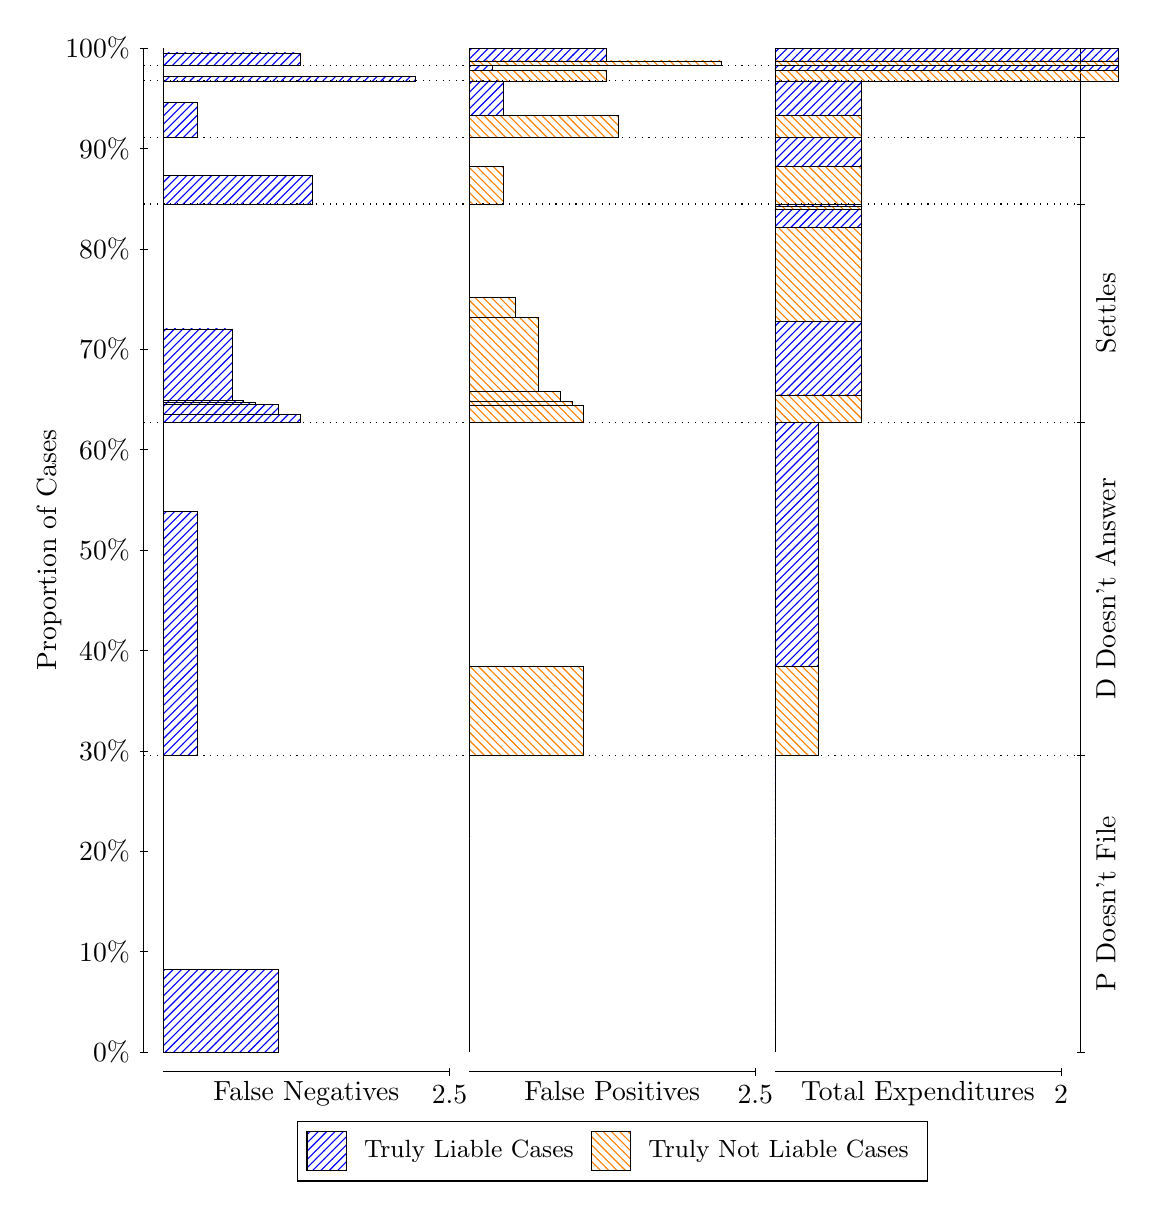
\begin{tikzpicture}
\draw[black, very thin] (1.5,1.75) -- (1.5,14.5);
\node[rotate=90, text=black, anchor=center] at (0.3, 8.125) {Proportion of Cases};
\draw[black, very thin] (1.45,1.75) -- (1.55,1.75);
\node[text=black, anchor=east] at (1.45, 1.75) {0\%};
\draw[black, very thin] (1.45,3.025) -- (1.55,3.025);
\node[text=black, anchor=east] at (1.45, 3.025) {10\%};
\draw[black, very thin] (1.45,4.3) -- (1.55,4.3);
\node[text=black, anchor=east] at (1.45, 4.3) {20\%};
\draw[black, very thin] (1.45,5.575) -- (1.55,5.575);
\node[text=black, anchor=east] at (1.45, 5.575) {30\%};
\draw[black, very thin] (1.45,6.85) -- (1.55,6.85);
\node[text=black, anchor=east] at (1.45, 6.85) {40\%};
\draw[black, very thin] (1.45,8.125) -- (1.55,8.125);
\node[text=black, anchor=east] at (1.45, 8.125) {50\%};
\draw[black, very thin] (1.45,9.4) -- (1.55,9.4);
\node[text=black, anchor=east] at (1.45, 9.4) {60\%};
\draw[black, very thin] (1.45,10.675) -- (1.55,10.675);
\node[text=black, anchor=east] at (1.45, 10.675) {70\%};
\draw[black, very thin] (1.45,11.95) -- (1.55,11.95);
\node[text=black, anchor=east] at (1.45, 11.95) {80\%};
\draw[black, very thin] (1.45,13.225) -- (1.55,13.225);
\node[text=black, anchor=east] at (1.45, 13.225) {90\%};
\draw[black, very thin] (1.45,14.5) -- (1.55,14.5);
\node[text=black, anchor=east] at (1.45, 14.5) {100\%};

\draw[black, very thin] (13.4,1.75) -- (13.4,14.5);
\draw[black, very thin] (13.35,1.75) -- (13.45,1.75);
\node[anchor=west] at (13.35, 1.75) {};
\draw[black, very thin] (13.35,5.5126) -- (13.45,5.5126);
\node[anchor=west] at (13.35, 5.5126) {};
\draw[black, very thin] (13.35,9.7493) -- (13.45,9.7493);
\node[anchor=west] at (13.35, 9.7493) {};
\draw[black, very thin] (13.35,12.519) -- (13.45,12.519);
\node[anchor=west] at (13.35, 12.519) {};
\draw[black, very thin] (13.35,13.364) -- (13.45,13.364);
\node[anchor=west] at (13.35, 13.364) {};
\draw[black, very thin] (13.35,14.082) -- (13.45,14.082);
\node[anchor=west] at (13.35, 14.082) {};
\draw[black, very thin] (13.35,14.275) -- (13.45,14.275);
\node[anchor=west] at (13.35, 14.275) {};
\draw[black, very thin] (13.35,14.5) -- (13.45,14.5);
\node[anchor=west] at (13.35, 14.5) {};

\draw[black, very thin, pattern color=blue, pattern=north east lines] (1.75,1.75) rectangle (3.2033,2.8035);
\draw[black, very thin, pattern color=orange, pattern=north west lines] (1.75,2.8035) rectangle (1.75,5.5126);
\draw[black, very thin, pattern color=blue, pattern=north east lines] (1.75,5.5126) rectangle (2.186,8.6184);
\draw[black, very thin, pattern color=orange, pattern=north west lines] (1.75,8.6184) rectangle (1.75,9.7493);
\draw[black, very thin, pattern color=blue, pattern=north east lines] (1.75,9.7493) rectangle (3.494,9.8482);
\draw[black, very thin, pattern color=blue, pattern=north east lines] (1.75,9.8482) rectangle (3.2033,9.9706);
\draw[black, very thin, pattern color=blue, pattern=north east lines] (1.75,9.9706) rectangle (2.9127,10.002);
\draw[black, very thin, pattern color=blue, pattern=north east lines] (1.75,10.002) rectangle (2.7673,10.028);
\draw[black, very thin, pattern color=blue, pattern=north east lines] (1.75,10.028) rectangle (2.622,10.934);
\draw[black, very thin, pattern color=orange, pattern=north west lines] (1.75,10.934) rectangle (1.75,12.519);
\draw[black, very thin, pattern color=blue, pattern=north east lines] (1.75,12.519) rectangle (3.6393,12.884);
\draw[black, very thin, pattern color=orange, pattern=north west lines] (1.75,12.884) rectangle (1.75,13.364);
\draw[black, very thin, pattern color=blue, pattern=north east lines] (1.75,13.364) rectangle (2.186,13.805);
\draw[black, very thin, pattern color=orange, pattern=north west lines] (1.75,13.805) rectangle (1.75,14.082);
\draw[black, very thin, pattern color=blue, pattern=north east lines] (1.75,14.082) rectangle (4.9473,14.144);
\draw[black, very thin, pattern color=orange, pattern=north west lines] (1.75,14.144) rectangle (1.75,14.275);
\draw[black, very thin, pattern color=blue, pattern=north east lines] (1.75,14.275) rectangle (3.494,14.438);
\draw[black, very thin, pattern color=orange, pattern=north west lines] (1.75,14.438) rectangle (1.75,14.5);
\draw[black, very thin, pattern color=orange, pattern=north west lines] (5.6333,1.75) rectangle (5.6333,4.4591);
\draw[black, very thin, pattern color=blue, pattern=north east lines] (5.6333,4.4591) rectangle (5.6333,5.5126);
\draw[black, very thin, pattern color=orange, pattern=north west lines] (5.6333,5.5126) rectangle (7.0867,6.6435);
\draw[black, very thin, pattern color=blue, pattern=north east lines] (5.6333,6.6435) rectangle (5.6333,9.7493);
\draw[black, very thin, pattern color=orange, pattern=north west lines] (5.6333,9.7493) rectangle (7.0867,9.9645);
\draw[black, very thin, pattern color=orange, pattern=north west lines] (5.6333,9.9645) rectangle (6.9413,10.011);
\draw[black, very thin, pattern color=orange, pattern=north west lines] (5.6333,10.011) rectangle (6.796,10.141);
\draw[black, very thin, pattern color=orange, pattern=north west lines] (5.6333,10.141) rectangle (6.5053,11.084);
\draw[black, very thin, pattern color=orange, pattern=north west lines] (5.6333,11.084) rectangle (6.2147,11.335);
\draw[black, very thin, pattern color=blue, pattern=north east lines] (5.6333,11.335) rectangle (5.6333,12.519);
\draw[black, very thin, pattern color=orange, pattern=north west lines] (5.6333,12.519) rectangle (6.0693,12.999);
\draw[black, very thin, pattern color=blue, pattern=north east lines] (5.6333,12.999) rectangle (5.6333,13.364);
\draw[black, very thin, pattern color=orange, pattern=north west lines] (5.6333,13.364) rectangle (7.5227,13.641);
\draw[black, very thin, pattern color=blue, pattern=north east lines] (5.6333,13.641) rectangle (6.0693,14.082);
\draw[black, very thin, pattern color=orange, pattern=north west lines] (5.6333,14.082) rectangle (7.3773,14.212);
\draw[black, very thin, pattern color=blue, pattern=north east lines] (5.6333,14.212) rectangle (5.924,14.275);
\draw[black, very thin, pattern color=orange, pattern=north west lines] (5.6333,14.275) rectangle (8.8307,14.337);
\draw[black, very thin, pattern color=blue, pattern=north east lines] (5.6333,14.337) rectangle (7.3773,14.5);
\draw[black, very thin, pattern color=orange, pattern=north west lines] (9.5167,1.75) rectangle (9.5167,4.4591);
\draw[black, very thin, pattern color=blue, pattern=north east lines] (9.5167,4.4591) rectangle (9.5167,5.5126);
\draw[black, very thin, pattern color=orange, pattern=north west lines] (9.5167,5.5126) rectangle (10.062,6.6435);
\draw[black, very thin, pattern color=blue, pattern=north east lines] (9.5167,6.6435) rectangle (10.062,9.7493);
\draw[black, very thin, pattern color=orange, pattern=north west lines] (9.5167,9.7493) rectangle (10.607,10.094);
\draw[black, very thin, pattern color=blue, pattern=north east lines] (9.5167,10.094) rectangle (10.607,11.031);
\draw[black, very thin, pattern color=orange, pattern=north west lines] (9.5167,11.031) rectangle (10.607,12.225);
\draw[black, very thin, pattern color=blue, pattern=north east lines] (9.5167,12.225) rectangle (10.607,12.446);
\draw[black, very thin, pattern color=orange, pattern=north west lines] (9.5167,12.446) rectangle (10.607,12.493);
\draw[black, very thin, pattern color=blue, pattern=north east lines] (9.5167,12.493) rectangle (10.607,12.519);
\draw[black, very thin, pattern color=orange, pattern=north west lines] (9.5167,12.519) rectangle (10.607,12.999);
\draw[black, very thin, pattern color=blue, pattern=north east lines] (9.5167,12.999) rectangle (10.607,13.364);
\draw[black, very thin, pattern color=orange, pattern=north west lines] (9.5167,13.364) rectangle (10.607,13.641);
\draw[black, very thin, pattern color=blue, pattern=north east lines] (9.5167,13.641) rectangle (10.607,14.082);
\draw[black, very thin, pattern color=orange, pattern=north west lines] (9.5167,14.082) rectangle (13.877,14.212);
\draw[black, very thin, pattern color=blue, pattern=north east lines] (9.5167,14.212) rectangle (13.877,14.275);
\draw[black, very thin, pattern color=orange, pattern=north west lines] (9.5167,14.275) rectangle (13.877,14.337);
\draw[black, very thin, pattern color=blue, pattern=north east lines] (9.5167,14.337) rectangle (13.877,14.5);
\draw[black, dotted] (1.5,5.5126) -- (13.4,5.5126);
\draw[black, dotted] (1.5,9.7493) -- (13.4,9.7493);
\draw[black, dotted] (1.5,12.519) -- (13.4,12.519);
\draw[black, dotted] (1.5,13.364) -- (13.4,13.364);
\draw[black, dotted] (1.5,14.082) -- (13.4,14.082);
\draw[black, dotted] (1.5,14.275) -- (13.4,14.275);
\draw[black, very thin] (1.75,1.5) -- (5.3833,1.5);
\node[text=black, anchor=north] at (3.5667, 1.5) {False Negatives};
\draw[black, very thin] (5.3833,1.45) -- (5.3833,1.55);
\node[text=black, anchor=north] at (5.3833, 1.45) {2.5};

\draw[black, very thin] (5.6333,1.5) -- (9.2667,1.5);
\node[text=black, anchor=north] at (7.45, 1.5) {False Positives};
\draw[black, very thin] (9.2667,1.45) -- (9.2667,1.55);
\node[text=black, anchor=north] at (9.2667, 1.45) {2.5};

\draw[black, very thin] (9.5167,1.5) -- (13.15,1.5);
\node[text=black, anchor=north] at (11.333, 1.5) {Total Expenditures};
\draw[black, very thin] (13.15,1.45) -- (13.15,1.55);
\node[text=black, anchor=north] at (13.15, 1.45) {2};

\node[text=black, centered, rotate=90] at (13.72, 3.6313) {P Doesn't File};
\node[text=black, centered, rotate=90] at (13.72, 7.6309) {D Doesn't Answer};
\node[text=black, centered, rotate=90] at (13.72, 11.134) {Settles};





\draw (7.449999999999999,1.5) node[draw=none] (baseCoordinate) {};
\begin{scope}[align=center]
        \matrix[scale=0.5, draw=black, below=0.5cm of baseCoordinate, nodes={draw}, column sep=0.1cm]{
            \node[rectangle, draw, minimum width=0.5cm, minimum height=0.5cm, pattern color=blue, pattern=north east lines] {}; &
            \node[draw=none, font=\small, text=black] (B) {Truly Liable Cases}; &
            \node[rectangle, draw, minimum width=0.5cm, minimum height=0.5cm, pattern color=orange, pattern=north west lines] {}; &
            \node[draw=none, font=\small, text=black] (B) {Truly Not Liable Cases}; \\
            };
\end{scope}

\end{tikzpicture}
\end{document}